\documentclass{article}
\usepackage[utf8]{inputenc}
\usepackage{graphicx}
\graphicspath{ {images/} }
\usepackage{enumitem}

%----------------------------------------------------------------------------------------
%	TITLE PAGE
%----------------------------------------------------------------------------------------

\newcommand*{\titleGP}{\begingroup
\centering 
\vspace*{\baselineskip}

\rule{\textwidth}{1.6pt}\vspace*{-\baselineskip}\vspace*{2pt}
\rule{\textwidth}{0.4pt}\\[\baselineskip]

{\LARGE CGIS Map Production\\ [0.3\baselineskip] Software Requirements Specification } \\ [0.2\baselineskip]
\rule{\textwidth}{0.4pt}\vspace*{-\baselineskip}\vspace{3.2pt}
\rule{\textwidth}{1.6pt}\\[\baselineskip] %

% \scshape %
% A concise specification on the functional requirements  \\
% and use cases of CGIS \\[\baselineskip]

% \vspace*{2\baselineskip}

Compiled By \\[\baselineskip]
{\Large Siyabonga Magubane - u15289347 \\ Bernard van Tonder -  u15008992 \\ Boikanyo Modiko - u15227678 \\ Cian Steenkamp - u15095682 \\ Robert Trankle - u15092454\par} 

\vfill

{\scshape 2017} \\[0.3\baselineskip]
{\large \#include}\par

\endgroup}

\begin{document}


\titleGP

\newpage
	
	\section{Introduction}
    	
        \subsection{Purpose}
        	{The purpose of this document is to put forth a description detailing the \textbf{CGIS Map Production}. It will explain the main purpose of the system, as well as additional subsystems, the interface of these systems, and what they will and will not do, as well as the constraints. Providing a detailed requirement specification of the system as a whole. It is intended for the Client, as well as developers who will integrate the system.}
    	\subsection{Scope}
{The CGIS Map Production will be a web-based application. It will create Statistical Maps(Thematic Maps), based on different attributes specified by a user. The maps will cover the Tshwane, and the different wards within Tshwane.\\\\
The system will provide a list of attributes,from a database, that the user may select. The selected attributes will allow the system to generate different types of Thematic Maps (Choropleth, Dot Density etc.) The system must be able to generate a minimum of 3 different Thematic maps.\\\\
The Standardisation sub-system will be the core of the system. It will take the information(data) from the database and standardise it in order to quantify the data for different regions.\\\\
This document aims to identify and outline various aspects of the CGIS Map Production system. The interfaces and operations will be discussed. It will also address the functional and non-functional requirements of the system, as well as the data requirements. This will outline the system, which will be used to derive a series of Use Cases.}
        \subsection{Definitions, Acronyms, and Abbreviations}
            \begin{table}[ht!]
	\centering
	\begin{tabular}{|p{4cm}|p{7cm}|}
		\hline
		\textbf{Term} & \textbf{Definition} \\		
		\hline
		UI & User interface \\
        \hline
		CRUD & Create, Read, Update and Delete \\
		\hline
		FR & Functional Requirement \\
		\hline
		GIS & Geographic Information System \\
		\hline
		CGIS & Center for Geographic Information System \\
		\hline
		UC & Use Case\\
		\hline
	\end{tabular}
\end{table}
            
            
        \subsection{References}
        {IEEE Recommended Practice for Software Requirements Specications\\
        2013-MSc-Rautenbach}
        \subsection{Overview}
	
	\section{Overall Description}
		
        \subsection{Product Perspective}
        
        	\subsubsection{System Interface}{
\textbf{User Interface}:\\\\
Functionality:\\\\
The functionality of the user interface is to allow the user to interact with the system. Through this aspect of the system the user can perform all the functions necessary to create and display a map. Through the interface the user will be able to create and display various thematic maps using the large geospatial dataset.\\\\
How functionality achieves requirements:\\\\
The user interface allows the functionality of the application to meet the requirements. The user is able to add geo-spatial database reference that has the source dataset using the UI. The user may select the display map option where three different maps will appear.The user may select the type of map they want to view and the map will be viewed in full, fulfilling the view automated map requirement.\\\\
\textbf{Hardware Interface}:\\\\
Functionality:\\\\
The functionality of this system interface is the physical hardware that allows software operation. The hardware in this case is specifically the mobile devices upon which the NavUP application will be installed.\\\\
How functionality achieves requirements :\\\\
This hardware will allow the achievement of the requirements by facilitating the operation of the application. The user will be able to press the physical device screen in order to operate the navigation and other such features of the application. The networking hardware of the components such as the wireless fidelity infrastructure within the device allows for communication to the system server. It is through this communication that the user's location can be determined and the system can function.\\\\
\textbf{Software Interface:}\\\\
Functionality:\\\\
The functionality of the software interface is to facilitate the communication between the hardware infrastructure of the devices running the application and the actual CGIS Map Pro=5u  application. An example of this would be the operating system of the device in use. The operating system would allow the application to make use of the Wi-Fi infrastructure and communicate the necessary information to the application. This would enable the device to communicate with the server and perform the necessary requests.\\\\
How functionality achieves requirements :\\\\
This would allow the achievement of the requirements as the communication of the application to the system server is vital to the operation of the NavUP system. By allowing communication over Wi-Fi the user's location can be determined, accounts can be logged in or created, information regarding heat mapping and general information can be retrieved by the user, fulfilling this requirement. Notifications can also be received by the users application through the Wi-Fi communication , fulfilling the this requirement .}

            \subsubsection{Communications Interface}
            \subsubsection{Memory}
            \subsubsection{Operations}
           
        
		\subsection{Product Functions}
    	\subsection{User Characteristics}
    	\subsection{Assumptions and Dependencies}
        
	\section{Specific Requirements}
    	\subsection{Functional Requirements}
        \begin{enumerate}[label=\alph*]
        \item Generate three different types of thematic maps.
		\item Allow the user to select attributes, that are available in the database, to generate the map.
		\item Display the three different types of thematic maps.
		\item Manipulate the scale of the map, to introduce
        \end{enumerate}
        \subsection{Quality(non-functional) Requirements}
        \begin{enumerate}[label=\alph*]
        \item Performance.
		\item Availability.
		\item Scalability.
		\item Identify (Intelligently) the best three maps to be displayed, based on attributes.
        \item Provide security (confidentiality) for the database and locations.\\
        \end{enumerate}
        Detailed Description:
        \begin{enumerate}[label=\alph*]
        \item Performance: Data will be input, maps rendered and displayed within a reasonable time. The software will immediately respond to user input. The process from input to output will endure for less than one minute. 
		\item Availability: The software will be functioning on demand with no obstructions to users who have sufficient permission.
		\item Scalability: Any complete dataset in the required format can be processed and displayed.
		\item Intelligence: Using artificial intelligence, the best three thematic maps for optimal information communication will be generated based on the input attributes.
        \item Security: Sensitive data will be protected. Only those with sufficient permission will be able to access sensitive data contained in the dataset.
        \end{enumerate}
        
	{
    \section{Use Cases}
\noindent\textbf{UC: Map Display and Scaling}

\begin{flushleft}
\begin{tabular}{ |p{7cm}|p{7cm}| } 
   \hline
  \multicolumn{2}{|p{\textwidth}|}{\textbf{Precondition:} The user should have generated the 3 maps by clicking "Generate Maps"} \\
  \hline
\textbf {Actor: General User} & \textbf{System: Navigation}\\ 
\hline
 & 0:System displays 3 types of thematic maps and a button for scaling each map\\ 
\hline
 1:The user scales the 3 maps by clicking on the appropriate "scaling" button  & 2: System displays scaled map(s) \\
  \hline
  \multicolumn{2}{|p{\textwidth}|}{\textbf{Postcondition: None}} \\
   \hline

\end{tabular}

\end{flushleft}
\begin{center}
    	Table 1: Find Current Location Use Case Narrative
\end{center}

\begin{figure}[h!]
	\includegraphics[width=\textwidth]{Graph_Display_and_Scaling}
	\caption{Graph Display and Scaling}
\end{figure}

\pagebreak

\noindent\textbf{UC2 Generate thematic maps}
\begin{flushleft}
\begin{tabular}{ |p{0.5\textwidth}|p{0.5\textwidth}| }
  \hline
  \multicolumn{2}{|p{\textwidth}|}{Precondition:} \\
  \hline
  Actor: User & System:  \\
   \hline
   & 0. System displays attributes for user to select \\
  \hline
    1.TUCBW user specifies the attributes they would like to use to generate the maps & 2. System generates 3 different types of thematic maps \\
  \hline
  3. TUCEW user clicks the Exit button & \\
  \hline
  \multicolumn{2}{|p{\textwidth}|}{Postcondition:} \\
   \hline
\end{tabular}
\end{flushleft}

\begin{figure}[h!]
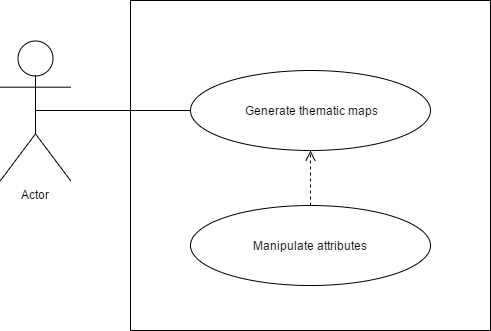
\includegraphics[width=\textwidth]{generate_maps_use_case}
	\caption{Use case diagram for generating thematic maps}
\end{figure}

\pagebreak

        \subsection{Performance Requirements}
        \subsection{Design Constraints}
        \subsection{Software System Attributes}
\end{document}